\clearpage

\section{Testable Predictions and Observational Signatures}
\label{sec:testable-predictions-and-observational-signatures}

Numerical estimates presented below are order-of-magnitude consistency
estimates derived from the geometric coupling between the~$\chi$
substrate and the effective relaxation fraction~$\Omega_\chi$.
Their role is to demonstrate that the framework operates within a
phenomenologically relevant regime.

\subsection{Hubble Constant from
\texorpdfstring{$\chi$}{χ} Dynamics}
\label{subsec:hubble-constant-from-chi-dynamics}

The Hubble parameter arises as an effective quantity:
\begin{equation}
  H(t) = \frac{\dot{\chi}}{\chi}.
\end{equation}
Assuming $\dot{\chi}_{\mathrm{eff}} \simeq c$, the present-day value is
$H_0 \simeq c/\chi(t_0)$.
Early- and late-universe probes sample~$\chi$ at different relaxation
stages, naturally leading to systematically different inferred values
of~$H_0$ without invoking additional cosmological components.

\paragraph{Resolution of the Hubble tension.}
The effective $H(z)$ acquires a mild redshift dependence departing from
$\Lambda$CDM at intermediate redshifts
($0.1 \lesssim z \lesssim 10$), testable through upcoming BAO and
supernova surveys.

\begin{figure}[t]
  \centering
  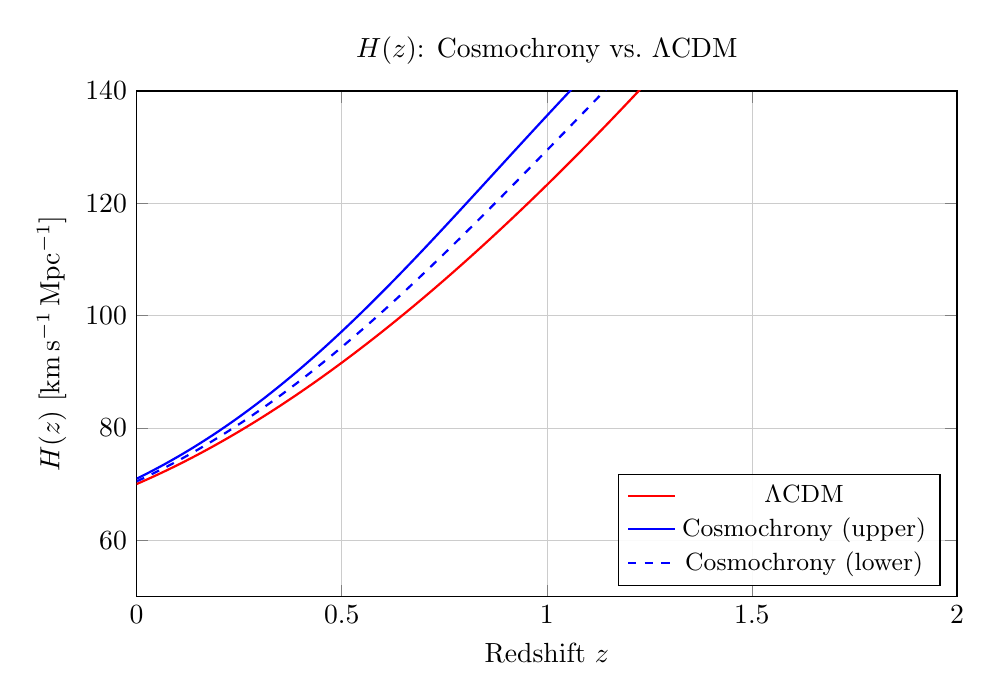
\begin{tikzpicture}
    \begin{axis}[
      width=12cm, height=8cm,
      title={$H(z)$: Cosmochrony vs.\ $\Lambda$CDM},
      xlabel={Redshift $z$},
      ylabel={$H(z)$ [km\,s$^{-1}$\,Mpc$^{-1}$]},
      xmin=0, xmax=2, ymin=50, ymax=140,
      xtick={0,0.5,1,1.5,2},
      legend style={
        at={(rel axis cs:0.98,0.02)},
        anchor=south east, draw=black,
        fill=white, fill opacity=0.9,
        text opacity=1, font=\small},
      grid=both,
      grid style={line width=.1pt, draw=gray!10},
      major grid style={line width=.2pt, draw=gray!40},
    ]
      \addplot[domain=0:2, samples=200,
        red, thick, mark=none]
        {70*sqrt(0.3*(1+x)^3 + 0.7)};
      \addlegendentry{$\Lambda$CDM}
      \addplot[domain=0:2, samples=200,
        blue, thick, mark=none]
        {70*sqrt(0.3*(1+x)^3+0.7)
          *(1+0.10*exp(-2*(x-1)^2))};
      \addlegendentry{Cosmochrony (upper)}
      \addplot[domain=0:2, samples=200,
        blue, thick, dashed, mark=none]
        {70*sqrt(0.3*(1+x)^3+0.7)
          *(1+0.05*exp(-2*(x-1)^2))};
      \addlegendentry{Cosmochrony (lower)}
    \end{axis}
  \end{tikzpicture}
  \caption{Schematic comparison of $H(z)$.
    Cosmochrony predicts a mild enhancement at intermediate
    redshifts due to relaxation inhomogeneities.}
  \label{fig:hubble-comparison}
\end{figure}

% ----------------------------------------------------------------------------
% Section 11.2 --- Redshift Drift
% From former §14.2, condensed
% ----------------------------------------------------------------------------
\subsection{Redshift Drift}
\label{subsec:redshift-drift}

Monotonic relaxation dynamics implies a slowly evolving cosmological
redshift.
The effective drift rate is
\begin{equation}
  \dot{z}_{\mathrm{eff}}
  \;\sim\;
  H_0 (1+z) - \frac{c}{\chi(t)},
\end{equation}
corresponding to a secular variation of order
$\Delta z \sim 10^{-10}\,\mathrm{yr}^{-1}$ at $z \sim 1$, differing
from $\Lambda$CDM at the $\sim 10\%$ level.
Future extremely large telescopes equipped with ultra-stable
spectrographs may probe this effect.

\subsection{Gravitational Wave Propagation}
  \label{subsec:gravitational-wave-propagation}

  In regions of high excitation density near compact objects, local
  suppression of~$\chi$ relaxation modifies the persistence and coherence
  of gravitational-wave projective descriptions.
  This effect induces frequency-dependent phase shifts or amplitude
  suppression, rather than purely dissipative losses.

  We predict a relative amplitude deviation from general relativistic
  templates scaling as
  \[
    \frac{\Delta A}{A}
    \sim \left(\frac{r_s}{r}\right)^2 ,
  \]
  where $r_s = 2GM/c^2$ is the Schwarzschild radius and $r$ the effective
  propagation radius of the dominant ringdown mode.

  For propagation at $r \approx 10\,r_s$, this yields
  \[
    \frac{\Delta A}{A} \sim 10^{-2} ,
  \]
  corresponding to a percent-level suppression of coherent gravitational-wave
  amplitudes relative to general relativity.

  This deviation should manifest most clearly during the late-time
  ringdown phase of binary black hole mergers as a systematic,
  frequency-dependent mismatch with general relativistic ringdown templates.
  The effect preserves luminal propagation speed but alters coherence
  structure.

  \textbf{Falsifiability condition.}
  If future high signal-to-noise detections ($\mathrm{SNR} \gtrsim 100$)
  by space-based observatories such as LISA constrain
  $\Delta A/A < 10^{-3}$ at $r \sim 10\,r_s$,
  the present scaling law would be excluded at the predicted amplitude level.

% ----------------------------------------------------------------------------
% Section 11.4 --- Galaxy Rotation Curves from Structural Relaxation
% From former §14.4, condensed
% ----------------------------------------------------------------------------
\subsection{Galaxy Rotation Curves from Structural Relaxation}
\label{subsec:galaxy-rotation-chi}

Persistent relaxation gradients in the $\chi$-substrate modify the
effective inertial response of orbiting matter, producing approximately
flat rotation curves without introducing dark matter components
(Section~\ref{subsec:phi-eff-galaxies}).
Observable consequences include a correlation between rotation curve
flattening and indicators of structural relaxation activity, deviations
from baryonic scaling relations in dynamically young galaxies, and a
reduced need for fine-tuned dark matter profiles in low-surface-brightness
systems.

% ----------------------------------------------------------------------------
% Section 11.5 --- Spin and Topological Signatures
% From former §14.5, condensed
% ----------------------------------------------------------------------------
\subsection{Spin and Topological Signatures}
\label{subsec:spin-and-topological-signatures}

If spin originates from topologically nontrivial configurations of~$\chi$
(Section~\ref{subsec:spin_topology}), ultra-high-precision interference
experiments sensitive to $4\pi$ rotational symmetry may probe deviations
associated with the internal topology of localized projectable
configurations.
Such deviations would appear as extremely small phase shifts under closed
$2\pi$ versus $4\pi$ rotational cycles.
These signatures are expected to be strongly suppressed and lie beyond
current experimental resolution.

\input{5-predictions_discussion_conclusion/11-testable-predictions-and-observational-signatures/006-dark-energy-absence}
\input{5-predictions_discussion_conclusion/11-testable-predictions-and-observational-signatures/007-cmb-polarization}
\subsection{Neutrino-Mediated Relaxation and Decay Signatures}
\label{subsec:neutrino-decay-signatures}

Particle decay and neutrino emission are manifestations of structural
reorganization
(Sections~\ref{subsec:metastability-and-decay},~\ref{subsec:neutrinos-partially-projectable-modes}).
Neutrino-like excitations act as non-local relaxation channels,
contributing to irreversible smoothing of admissible configurations.

\subsubsection*{Environmental Modulation of Particle Stability}
\label{subsec:environmental-decay-modulation}

\subsection{Environmental Modulation of Particle Lifetimes}
\label{subsec:environmental-modulation-lifetimes}

Particle stability may exhibit a weak environmental dependence.
At leading order:
\begin{equation}
  \frac{\delta \Gamma}{\Gamma}
  \;\simeq\;
  \beta \, \frac{\Delta U}{c^{2}},
  \label{eq:lifetime-modulation}
\end{equation}
where $\beta \lesssim 10^{-6}$ (from local position invariance
constraints) and
$\Delta U / c^{2} \sim 10^{-7}$--$10^{-6}$ for typical galactic
environments, yielding
\begin{equation}
  \frac{\delta \tau}{\tau}
  \;\sim\;
  10^{-13} \text{--} 10^{-12},
  \label{eq:lifetime-order-of-magnitude}
\end{equation}
well below current sensitivities but conceptually distinct from standard
effects.
The cleanest experimental target is leptonic weak decay; the most
amplified interferometric target is neutral-meson mixing.
Near compact objects
($\Delta U/c^2 \sim 10^{-4}$), the effect rises to
$\delta\tau/\tau \sim 10^{-10}$, manifesting as environment-correlated
spectral biases in hadronic cascades.

\subsection{Strong Gravitational Lensing}
\label{subsec:strong-gravitational-lensing}

The effective lensing potential decomposes as
$\Phi_{\mathrm{eff}} = \Phi_{\mathrm{bar}} + \Phi_{\chi}$,
with convergence
\begin{equation}
  \kappa(\boldsymbol{\theta})
  = \frac{D_l D_{ls}}{c^2 D_s}
    \int \nabla_\perp^2
    \Phi_{\mathrm{eff}}\!
      \left(D_l\boldsymbol{\theta},z\right)\,dz ,
\end{equation}
yielding $\kappa = \kappa_{\mathrm{bar}} + \kappa_{\chi}$.
The emergent contribution is parametrized as
\begin{equation}
  \Phi_{\chi}(\mathbf{x})
  = \frac{c^2}{2}\,
    \ln\!\left(
      \frac{K(\bar\chi(\mathbf{x}))}{K_\infty}
    \right).
\end{equation}
Testable signatures include partial decorrelation between baryonic mass
and lensing strength, enhanced sensitivity to cluster morphology, strong
lensing without dark matter substructure, and redshift dependence tracing
relaxation rather than mass accretion history.

\subsubsection*{Early Massive Structures in the JWST Era}
\label{subsec:jwst-early-structures}

Massive galaxies and strong lensing at $z \gtrsim 8$ are naturally
accommodated: effective mass reflects localized resistance to relaxation
associated with spectrally robust projected configurations, rather than
requiring rapid hierarchical assembly.

\subsubsection*{``Impossibly Early'' Galaxies}
\label{subsec:impossibly-early-galaxies}

Their large effective masses encode strong resistance to relaxation rather
than cumulative accretion.
Cosmochrony predicts that such galaxies should exhibit relatively stable
effective masses over extended redshift intervals, contrasting with the
rapid growth required in hierarchical scenarios.

\subsubsection*{Qualitative Predictions}
\label{subsec:qualitative-prediction-early-galaxies}
\label{subsec:qualitative-prediction-early-lensing}

Massive galaxies at $z \gtrsim 8$ should persist with only moderate mass
evolution.
Early strong-lensing configurations should display weak redshift evolution
of their effective convergence, with an early onset followed by moderate
evolution.

\subsubsection*{Strong Gravitational Lensing in Abell-1689}
\label{subsec:a1689-strong-lensing}

The emergent convergence is isolated as
\begin{equation}
  \kappa_{\chi}(\boldsymbol{\theta})
  = \kappa_{\mathrm{eff}}(\boldsymbol{\theta})
    - \kappa_{\mathrm{bar}}(\boldsymbol{\theta}),
\end{equation}
with the emergent lensing potential obtained from
$\nabla_{\boldsymbol{\theta}}^2 \psi_{\chi} =
  2\kappa_{\chi}$.
In Cosmochrony, $\kappa_{\chi}$ is emergent geometric focusing from
collective $\chi$-substrate constraints, not additional dark matter.

  \subsubsection*{Quantitative Scaling and Falsifiability}

    Beyond qualitative decorrelation effects, the emergent contribution
    $\kappa_{\chi}$ admits an order-of-magnitude scaling in saturated
    cluster cores.

    We parameterize the relative excess convergence as
    \begin{equation}
      \frac{\kappa_{\chi}}{\kappa_{\mathrm{bar}}}
      \sim \gamma
      \left(
        \frac{\Sigma_{\mathrm{bar}}}
        {\Sigma_*}
      \right),
    \end{equation}
    where $\Sigma_{\mathrm{bar}}$ is the baryonic surface density,
    $\Sigma_*$ denotes a characteristic structural relaxation scale of
    the $\chi$ substrate, and $\gamma$ is a dimensionless response
    coefficient encoding substrate efficiency.

    For massive clusters with
    $\Sigma_{\mathrm{bar}} \sim \Sigma_*$,
    this yields
    \begin{equation}
      \frac{\kappa_{\chi}}{\kappa_{\mathrm{bar}}}
      \sim \gamma ,
    \end{equation}
    with a natural expectation
    $\gamma \sim 10^{-2} \text{--} 10^{-1}$,
    corresponding to percent-to-ten-percent level decorrelation
    between baryonic mass distribution and total lensing convergence.

    This deviation should manifest as a systematic mismatch between
    high-resolution baryonic mass reconstructions and gravitational
    lensing maps, particularly in morphologically complex cluster cores
    such as Abell-1689.

    \textbf{Falsifiability condition.}
    If future lensing reconstructions constrain
    $\kappa_{\chi}/\kappa_{\mathrm{bar}} < 10^{-2}$
    in saturated cluster environments, the present scaling law
    would be excluded at the predicted amplitude level.

\input{5-predictions_discussion_conclusion/11-testable-predictions-and-observational-signatures/010-experimental-outlook}
\input{5-predictions_discussion_conclusion/11-testable-predictions-and-observational-signatures/011-summary-predictions}
